%======================================================
% CHAPTER II: SWP - SOFTWARE PROJECT MANAGEMENT PLAN
%======================================================
\chapter{SWP -- KẾ HOẠCH QUẢN LÝ DỰ ÁN PHẦN MỀM}

\section{Tổng quan Kế hoạch Dự án}

Chương này trình bày \textbf{Kế hoạch Quản lý Dự án Phần mềm (Software Project Management Plan -- SWP)} cho hệ thống Chatbot hỗ trợ học tập ứng dụng RAG. Tài liệu này bao gồm phạm vi dự án, ước lượng công sức, phân tích rủi ro, kế hoạch tiến độ, quy trình phát triển và quản lý cấu hình mã nguồn.

\begin{table}[H]
  \centering
  \caption{Thông tin chung dự án}
  \label{tab:project-info}
  \renewcommand{\arraystretch}{1.4}
  \begin{tabularx}{\textwidth}{|l|X|}
    \hline
    \rowcolor{blue!10}
    \textbf{Thông tin} & \textbf{Chi tiết} \\
    \hline
    Tên dự án & Xây dựng Hệ thống Chatbot Hỗ trợ Học tập ứng dụng RAG \\
    \hline
    Môn học & Công nghệ Phần mềm \\
    \hline
    Giảng viên hướng dẫn & Thầy Nguyễn Văn Chiến \\
    \hline
    Nhóm thực hiện & Nhóm 9 (7 thành viên) \\
    \hline
    Thời gian thực hiện & Tháng 3 -- Tháng 7 năm 2026 \\
    \hline
    Phương pháp quản lý & Agile Scrum (8 Sprint, 2 tuần/Sprint) \\
    \hline
    Công cụ quản lý & Jira Software, GitHub \\
    \hline
  \end{tabularx}
\end{table}

\section{Phạm vi Dự án}

\subsection{Phát biểu Phạm vi}

Dự án xây dựng một hệ thống Chatbot thông minh ứng dụng kỹ thuật RAG phục vụ sinh viên và quản trị viên trong môi trường học tập. Hệ thống bao gồm:
\begin{itemize}[itemsep=3pt]
  \item \textbf{Frontend:} Giao diện ReactJS với Chat Sandbox, quản lý tài liệu và Dashboard Benchmark.
  \item \textbf{Backend:} REST API FastAPI xử lý toàn bộ nghiệp vụ RAG, Embedding và LLM.
  \item \textbf{AI Pipeline:} Ingestion Pipeline (Chunking + Embedding) và RAG Pipeline (Retrieval + Generation).
  \item \textbf{Database:} ChromaDB (Vector) + MySQL (Quan hệ).
  \item \textbf{Benchmark Module:} Đánh giá định lượng các cấu hình RAG theo RAGAS.
\end{itemize}

\subsection{Sản phẩm Bàn giao (Deliverables)}

\begin{table}[H]
  \centering
  \caption{Danh sách sản phẩm bàn giao}
  \label{tab:deliverables}
  \renewcommand{\arraystretch}{1.4}
  \begin{tabularx}{\textwidth}{|c|l|X|l|}
    \hline
    \rowcolor{blue!10}
    \textbf{STT} & \textbf{Sản phẩm} & \textbf{Mô tả} & \textbf{Thời hạn} \\
    \hline
    1 & SWP Document & Kế hoạch quản lý dự án & Sprint 1 \\
    \hline
    2 & SWR Document & Đặc tả yêu cầu phần mềm & Sprint 2 \\
    \hline
    3 & SWD Document & Tài liệu thiết kế phần mềm & Sprint 3 \\
    \hline
    4 & Source Code & Backend FastAPI + Frontend ReactJS & Sprint 6 \\
    \hline
    5 & SWT Document & Báo cáo kiểm thử + Benchmark & Sprint 7 \\
    \hline
    6 & Final Report & Báo cáo tổng hợp LaTeX & Sprint 8 \\
    \hline
  \end{tabularx}
\end{table}

\section{Ước lượng Công sức và Tài nguyên}

\subsection{Ước lượng Công sức}

\begin{table}[H]
  \centering
  \caption{Ước lượng công sức theo module}
  \label{tab:effort}
  \renewcommand{\arraystretch}{1.4}
  \begin{tabularx}{\textwidth}{|c|l|X|c|c|}
    \hline
    \rowcolor{blue!10}
    \textbf{STT} & \textbf{Module} & \textbf{Công việc chính} & \textbf{Người} & \textbf{Tuần} \\
    \hline
    1 & Backend FastAPI & API design, RAG pipeline, Auth & 2 & 6 \\
    \hline
    2 & Frontend ReactJS & UI/UX, Chat, Dashboard & 2 & 6 \\
    \hline
    3 & AI/ML Pipeline & Embedding, ChromaDB, LLM & 2 & 5 \\
    \hline
    4 & Benchmark Module & Test framework, RAGAS metrics & 1 & 4 \\
    \hline
    5 & Database & MySQL schema, ChromaDB setup & 1 & 3 \\
    \hline
    6 & Testing & Test cases, kiểm thử tích hợp & 2 & 3 \\
    \hline
    7 & Documentation & SWP/SWR/SWD/SWT + báo cáo & 2 & 4 \\
    \hline
  \end{tabularx}
\end{table}

\subsection{Phân công Nhân sự (RACI Matrix)}

\begin{table}[H]
  \centering
  \caption{Ma trận phân công trách nhiệm (RACI)}
  \label{tab:raci}
  \renewcommand{\arraystretch}{1.4}
  \begin{tabularx}{\textwidth}{|l|c|c|c|c|c|c|c|}
    \hline
    \rowcolor{blue!10}
    \textbf{Công việc} & \textbf{Hưng} & \textbf{Danh} & \textbf{Đạt H} & \textbf{Khánh} & \textbf{Dũng} & \textbf{Đạt L} & \textbf{Trinh} \\
    \hline
    Thiết kế hệ thống & R & C & C & I & I & I & I \\
    \hline
    Backend FastAPI & R & A & C & I & C & I & I \\
    \hline
    Frontend ReactJS & I & I & R & A & C & I & C \\
    \hline
    RAG Pipeline & A & R & I & C & I & C & I \\
    \hline
    ChromaDB \& DB & I & A & I & R & I & C & I \\
    \hline
    Benchmark Module & C & I & I & I & R & A & I \\
    \hline
    Kiểm thử & I & I & C & C & I & I & R \\
    \hline
    Tài liệu báo cáo & A & C & I & I & I & C & R \\
    \hline
    \multicolumn{8}{l}{\small R=Responsible, A=Accountable, C=Consulted, I=Informed} \\
  \end{tabularx}
\end{table}

\section{Quy trình Phát triển -- Agile Scrum}

\subsection{Giới thiệu Agile Scrum}

Nhóm áp dụng phương pháp Agile Scrum với các đặc điểm:
\begin{itemize}[itemsep=3pt]
  \item \textbf{Sprint:} Chu kỳ phát triển 2 tuần/sprint, tổng 8 sprint (16 tuần).
  \item \textbf{Daily Standup:} Họp ngắn hàng ngày báo cáo tiến độ.
  \item \textbf{Sprint Review:} Kiểm tra sản phẩm cuối sprint với giảng viên.
  \item \textbf{Sprint Retrospective:} Rút kinh nghiệm để cải thiện quy trình.
  \item \textbf{Product Backlog:} Toàn bộ User Story được quản lý trên Jira.
\end{itemize}

\subsection{Quy trình Làm việc}

Mỗi công việc trên Jira trải qua các trạng thái:

\begin{center}
  \begin{tikzpicture}[
    node distance=0.8cm,
    box/.style={rectangle, rounded corners=4pt, draw=blue!60, fill=blue!8,
                text width=2cm, align=center, minimum height=0.8cm, font=\small},
    arrow/.style={-Stealth, thick, blue!70}
  ]
    \node[box] (backlog) {Backlog};
    \node[box, right=of backlog] (todo) {To Do};
    \node[box, right=of todo] (inprog) {In Progress};
    \node[box, right=of inprog] (review) {Code Review};
    \node[box, right=of review] (test) {Testing};
    \node[box, right=of test] (done) {Done};

    \draw[arrow] (backlog) -- (todo);
    \draw[arrow] (todo) -- (inprog);
    \draw[arrow] (inprog) -- (review);
    \draw[arrow] (review) -- (test);
    \draw[arrow] (test) -- (done);
  \end{tikzpicture}
\end{center}

\subsection{Kế hoạch Sprint}

\begin{table}[H]
  \centering
  \caption{Kế hoạch Sprint dự án}
  \label{tab:sprint-plan}
  \renewcommand{\arraystretch}{1.4}
  \begin{tabularx}{\textwidth}{|c|X|l|l|}
    \hline
    \rowcolor{blue!10}
    \textbf{Sprint} & \textbf{Nội dung chính} & \textbf{Thời gian} & \textbf{Trạng thái} \\
    \hline
    Sprint 1 & Phân tích yêu cầu, thiết kế kiến trúc hệ thống, viết SWP/SWR & Tuần 1--2 & \textcolor{green!60!black}{Hoàn thành} \\
    \hline
    Sprint 2 & Thiết kế CSDL, vẽ biểu đồ UML, viết SWD & Tuần 3--4 & \textcolor{green!60!black}{Hoàn thành} \\
    \hline
    Sprint 3 & Xây dựng Backend FastAPI (CRUD, Auth, API cơ bản) & Tuần 5--6 & \textcolor{green!60!black}{Hoàn thành} \\
    \hline
    Sprint 4 & Xây dựng Frontend ReactJS (Chat UI, Upload) & Tuần 7--8 & \textcolor{green!60!black}{Hoàn thành} \\
    \hline
    Sprint 5 & Tích hợp ChromaDB, RAG Pipeline, LLM API & Tuần 9--10 & \textcolor{green!60!black}{Hoàn thành} \\
    \hline
    Sprint 6 & Module Benchmark, Dashboard, tích hợp đầy đủ & Tuần 11--12 & \textcolor{green!60!black}{Hoàn thành} \\
    \hline
    Sprint 7 & Kiểm thử hệ thống, chạy Benchmark RAGAS & Tuần 13--14 & \textcolor{green!60!black}{Hoàn thành} \\
    \hline
    Sprint 8 & Hoàn thiện báo cáo LaTeX, review và submit & Tuần 15--16 & \textcolor{green!60!black}{Hoàn thành} \\
    \hline
  \end{tabularx}
\end{table}

\section{Quản lý Backlog}

\subsection{Danh sách Epic}

Các Epic chính của dự án bao gồm:
\begin{itemize}[itemsep=3pt]
  \item \textbf{EP-01:} Xây dựng Backend FastAPI
  \item \textbf{EP-02:} Xây dựng Frontend ReactJS
  \item \textbf{EP-03:} Xây dựng AI/RAG Pipeline
  \item \textbf{EP-04:} Tích hợp ChromaDB \& MySQL
  \item \textbf{EP-05:} Module Benchmark \& RAGAS
  \item \textbf{EP-06:} Thiết kế giao diện \& UX
  \item \textbf{EP-07:} Kiểm thử hệ thống
  \item \textbf{EP-08:} Viết tài liệu báo cáo
\end{itemize}

\subsection{Một số User Story tiêu biểu}

\begin{table}[H]
  \centering
  \caption{Danh sách User Story tiêu biểu}
  \label{tab:user-stories}
  \renewcommand{\arraystretch}{1.4}
  \begin{tabularx}{\textwidth}{|l|l|X|c|}
    \hline
    \rowcolor{blue!10}
    \textbf{ID} & \textbf{Vai trò} & \textbf{User Story} & \textbf{Story Points} \\
    \hline
    US-01 & Sinh viên & Đặt câu hỏi và nhận câu trả lời từ Chatbot dựa trên tài liệu môn học. & 8 \\
    \hline
    US-02 & Sinh viên & Xem lịch sử hội thoại và tiếp tục ngữ cảnh trò chuyện. & 5 \\
    \hline
    US-03 & Sinh viên & Cấu hình thông số RAG (Top-K, Chunking, Embedding) trong Sandbox. & 8 \\
    \hline
    US-04 & Quản trị viên & Tải lên tài liệu PDF/DOCX và theo dõi trạng thái xử lý. & 8 \\
    \hline
    US-05 & Quản trị viên & Quản lý, xóa, cập nhật tài liệu trong kho tri thức. & 5 \\
    \hline
    US-06 & Quản trị viên & Chạy Benchmark với nhiều cấu hình RAG khác nhau. & 13 \\
    \hline
    US-07 & Quản trị viên & Xem Dashboard tổng quan hiệu năng qua biểu đồ Radar. & 8 \\
    \hline
    US-08 & Hệ thống & Tự động phân mảnh và tạo Vector Embedding khi tài liệu được tải lên. & 13 \\
    \hline
  \end{tabularx}
\end{table}

\subsection{Minh họa Product Backlog trên Jira}

\begin{figure}[H]
  \centering
  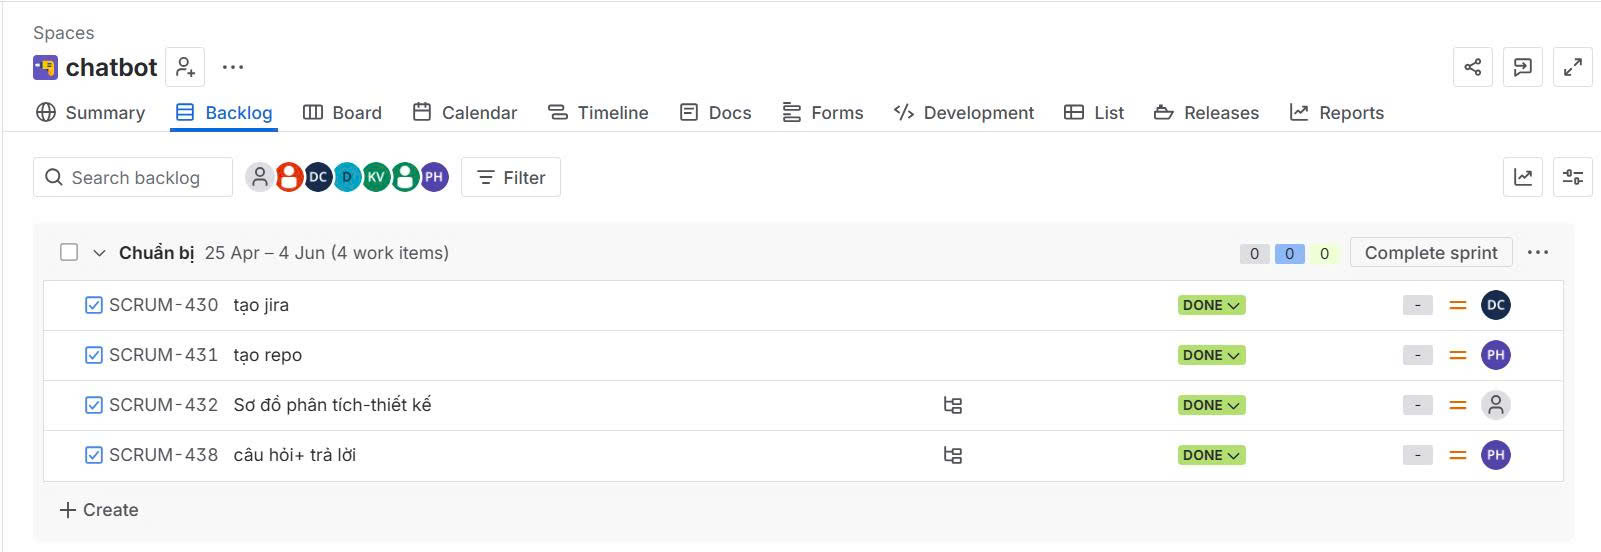
\includegraphics[width=\textwidth]{images/backlog_1.jpg}
  \caption{Product Backlog trên Jira (Phần 1)}
  \label{fig:backlog1}
\end{figure}

\begin{figure}[H]
  \centering
  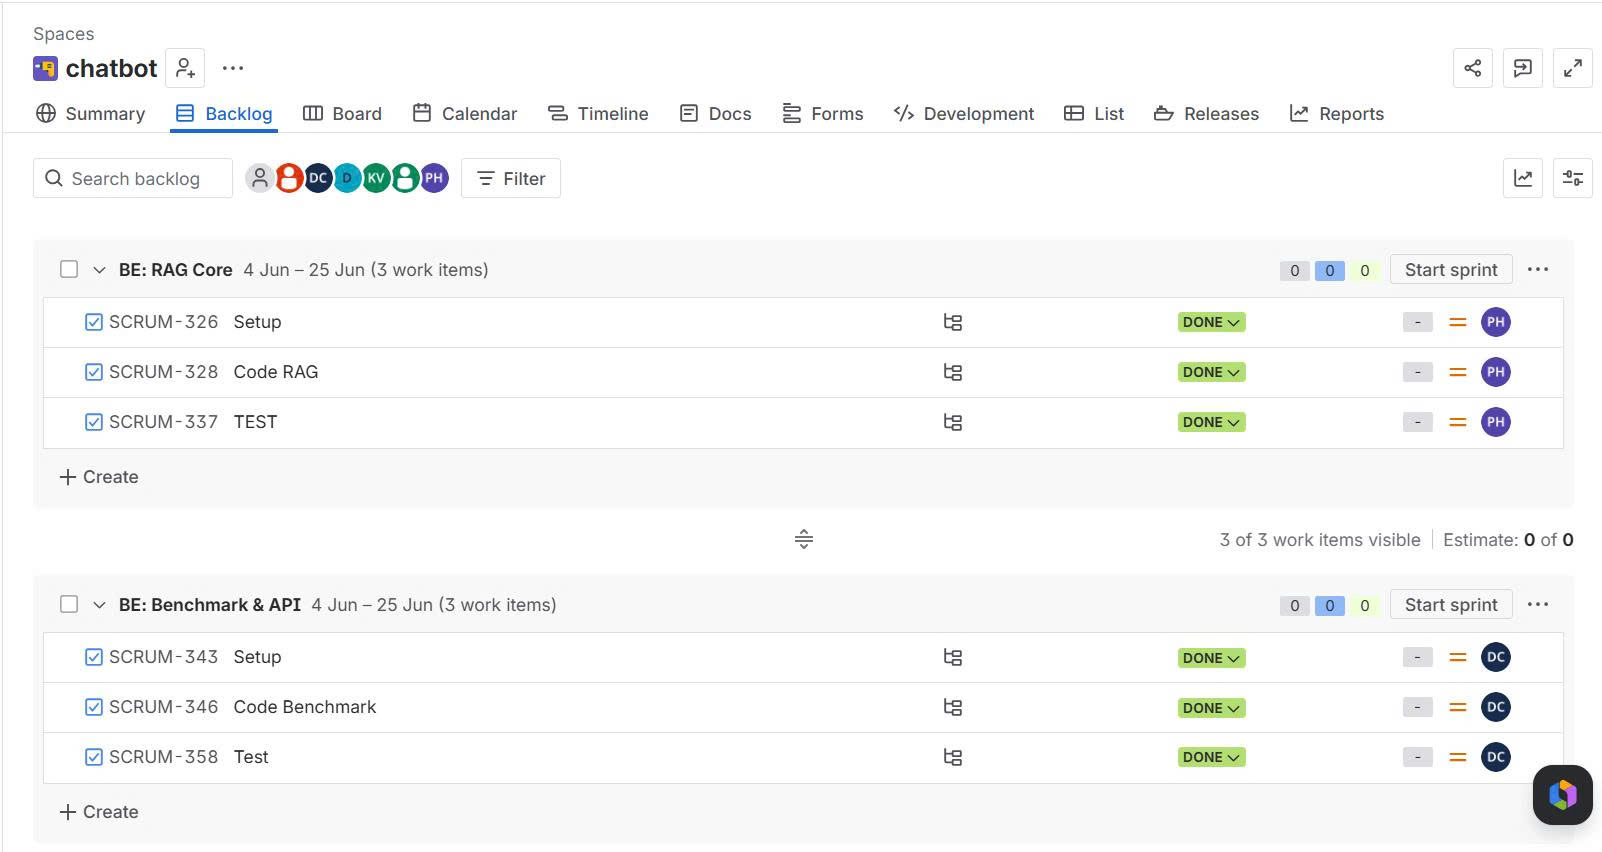
\includegraphics[width=\textwidth]{images/backlog_2.jpg}
  \caption{Product Backlog trên Jira (Phần 2)}
  \label{fig:backlog2}
\end{figure}

\begin{figure}[H]
  \centering
  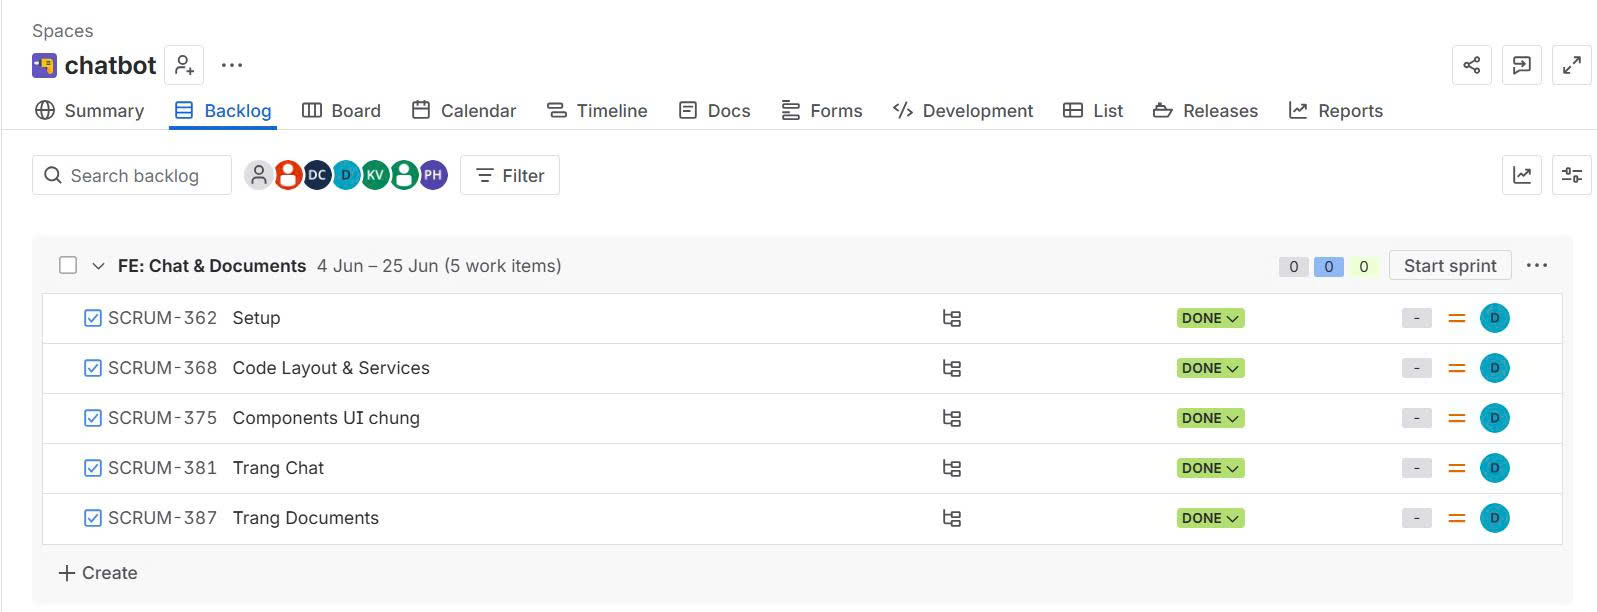
\includegraphics[width=\textwidth]{images/backlog_3.jpg}
  \caption{Product Backlog trên Jira (Phần 3)}
  \label{fig:backlog3}
\end{figure}

\begin{figure}[H]
  \centering
  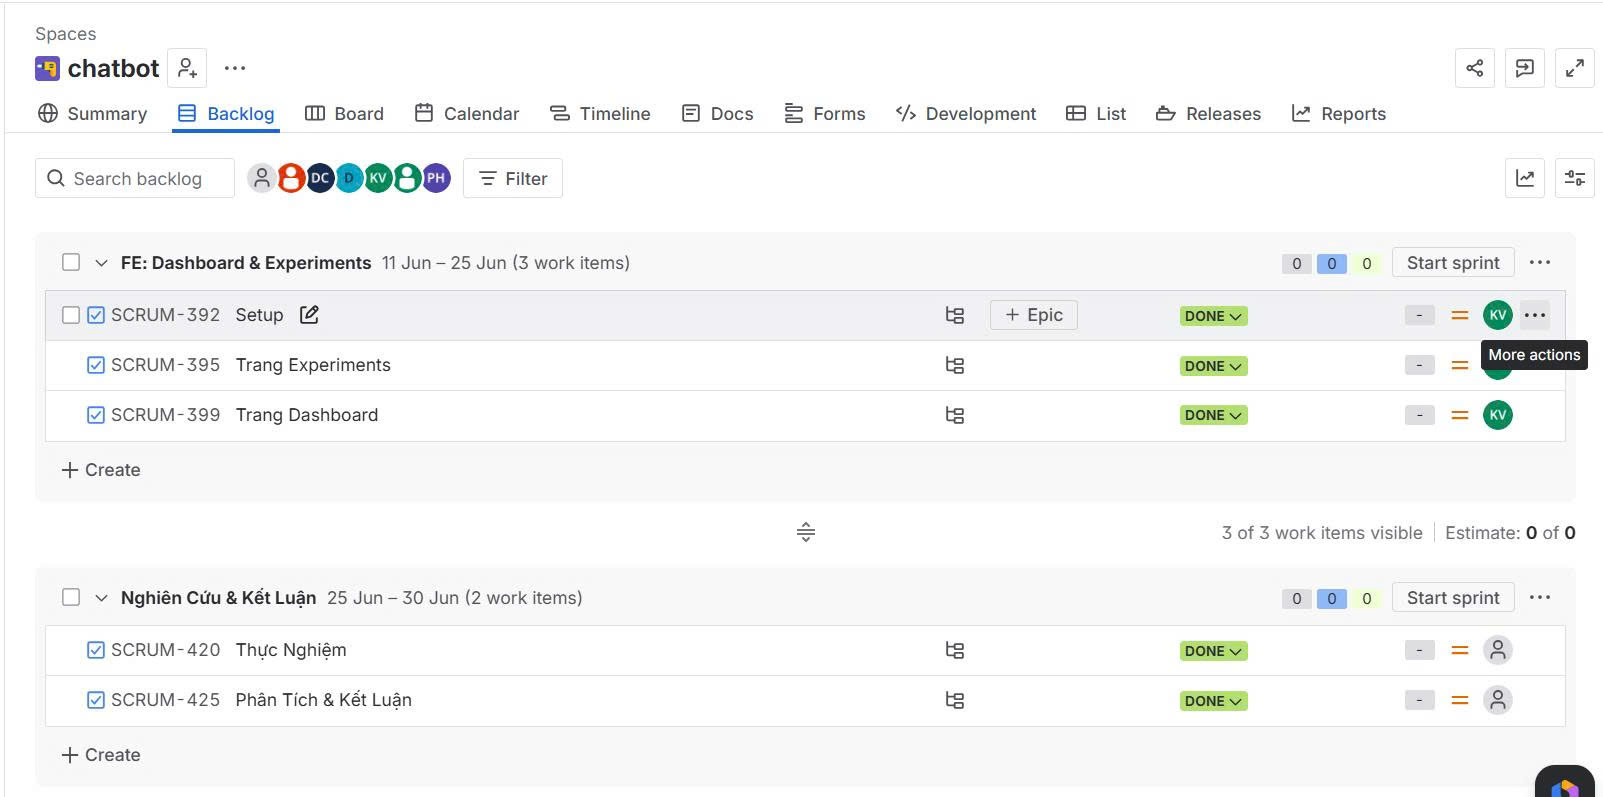
\includegraphics[width=\textwidth]{images/backlog_4.jpg}
  \caption{Product Backlog trên Jira (Phần 4)}
  \label{fig:backlog4}
\end{figure}

\begin{figure}[H]
  \centering
  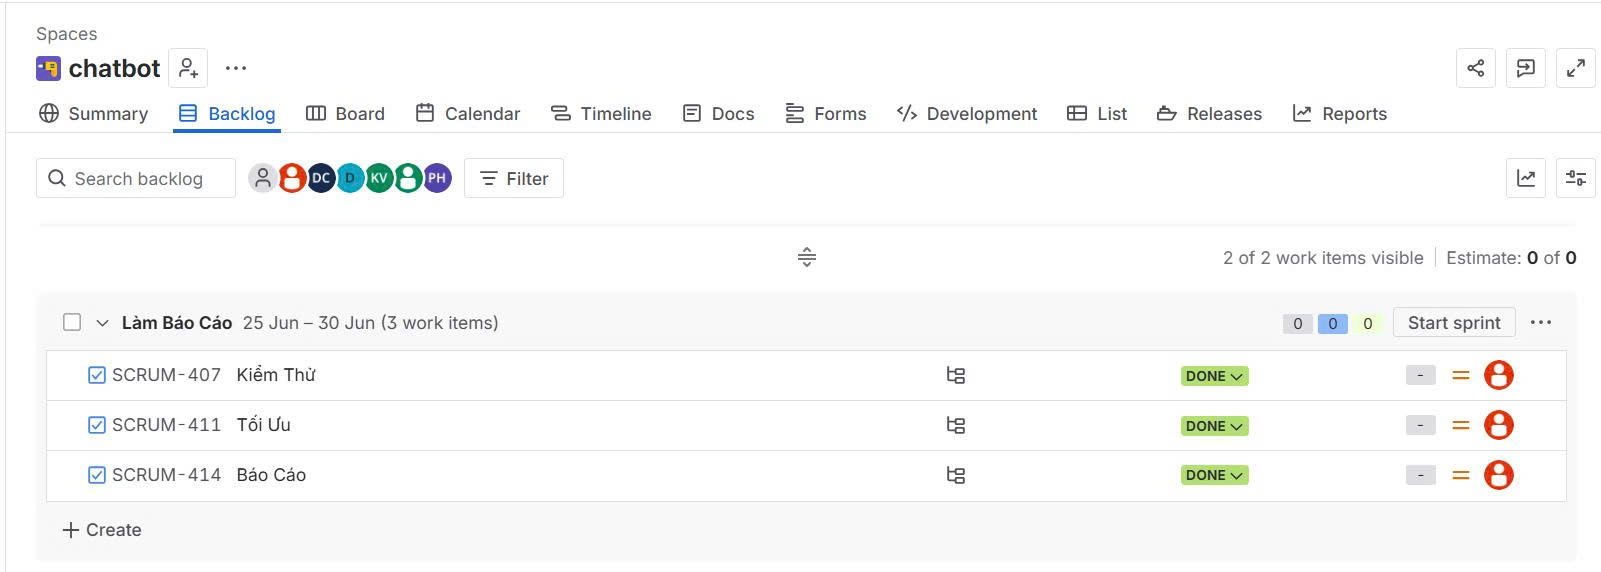
\includegraphics[width=\textwidth]{images/backlog_5.jpg}
  \caption{Product Backlog trên Jira (Phần 5)}
  \label{fig:backlog5}
\end{figure}

\subsection{Bảng Kanban Quản lý Công việc}

\begin{figure}[H]
  \centering
  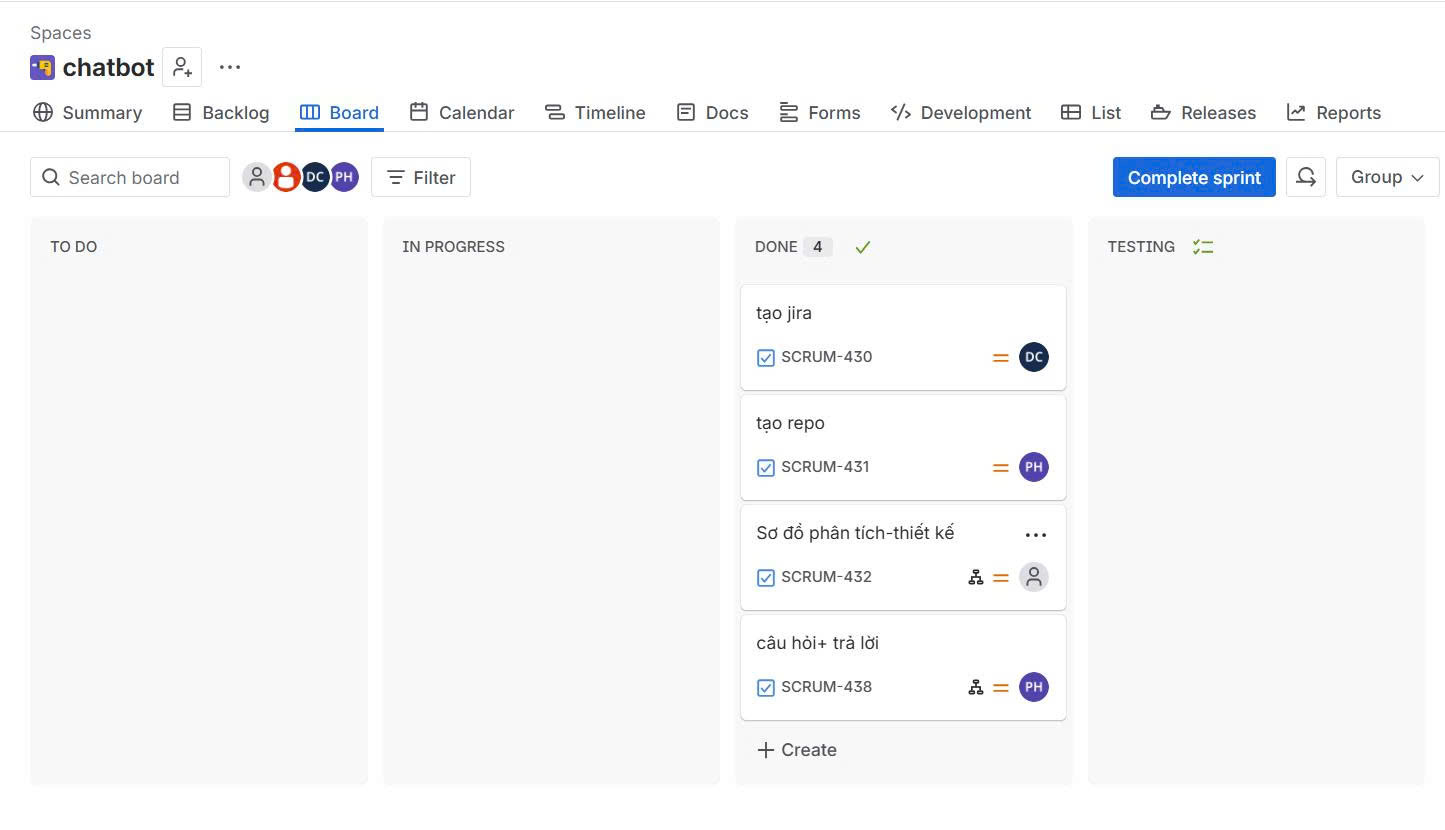
\includegraphics[width=\textwidth]{images/jira_board.png}
  \caption{Bảng Kanban quản lý công việc trên Jira}
  \label{fig:jira-board}
\end{figure}

Hình \ref{fig:jira-board} thể hiện toàn bộ bảng Kanban của dự án. Mỗi thẻ (Card) đại diện cho một nhiệm vụ cụ thể và được di chuyển giữa các cột tương ứng với trạng thái công việc trong suốt vòng đời phát triển phần mềm.

\section{Phân tích Rủi ro}

\begin{table}[H]
  \centering
  \caption{Ma trận phân tích rủi ro dự án}
  \label{tab:risk}
  \renewcommand{\arraystretch}{1.5}
  \begin{tabularx}{\textwidth}{|c|X|c|c|X|}
    \hline
    \rowcolor{blue!10}
    \textbf{ID} & \textbf{Rủi ro} & \textbf{Xác suất} & \textbf{Tác động} & \textbf{Biện pháp giảm thiểu} \\
    \hline
    R01 & API LLM (Gemini) bị giới hạn rate limit & Cao & Cao & Implement retry logic và caching kết quả. \\
    \hline
    R02 & Hiệu suất ChromaDB chậm với lượng tài liệu lớn & Trung bình & Cao & Tối ưu chunking size, sử dụng batch embedding. \\
    \hline
    R03 & Thành viên nhóm không đồng bộ tiến độ & Cao & Trung bình & Scrum daily standup, review code pull request. \\
    \hline
    R04 & Kết quả Benchmark không ổn định & Trung bình & Trung bình & Chạy benchmark nhiều lần, lấy trung bình. \\
    \hline
    R05 & Tài liệu tải lên có format phức tạp (bảng, hình) & Cao & Trung bình & Sử dụng pdfplumber kết hợp OCR fallback. \\
    \hline
    R06 & Xung đột code khi merge & Trung bình & Thấp & Branch strategy rõ ràng, PR review bắt buộc. \\
    \hline
  \end{tabularx}
\end{table}

\section{Quản lý Cấu hình -- GitHub}

\subsection{Chiến lược Nhánh (Branch Strategy)}

Nhóm áp dụng chiến lược nhánh \textbf{Git Flow} với cấu trúc:
\begin{itemize}[itemsep=3pt]
  \item \textbf{main:} Nhánh chính, chỉ nhận code đã được review và test đầy đủ.
  \item \textbf{develop:} Nhánh tích hợp, tổng hợp code từ các feature branch.
  \item \textbf{feature/[tên-feature]:} Nhánh phát triển tính năng (ví dụ: \texttt{feature/rag-pipeline}).
  \item \textbf{hotfix/[tên-fix]:} Nhánh sửa lỗi khẩn cấp.
\end{itemize}

Quy trình: \texttt{feature branch} $\rightarrow$ \textbf{Pull Request} $\rightarrow$ \textbf{Code Review} (tối thiểu 1 reviewer) $\rightarrow$ \texttt{develop} $\rightarrow$ \texttt{main}.

\subsection{Cấu trúc Repository}

\begin{figure}[H]
  \centering
  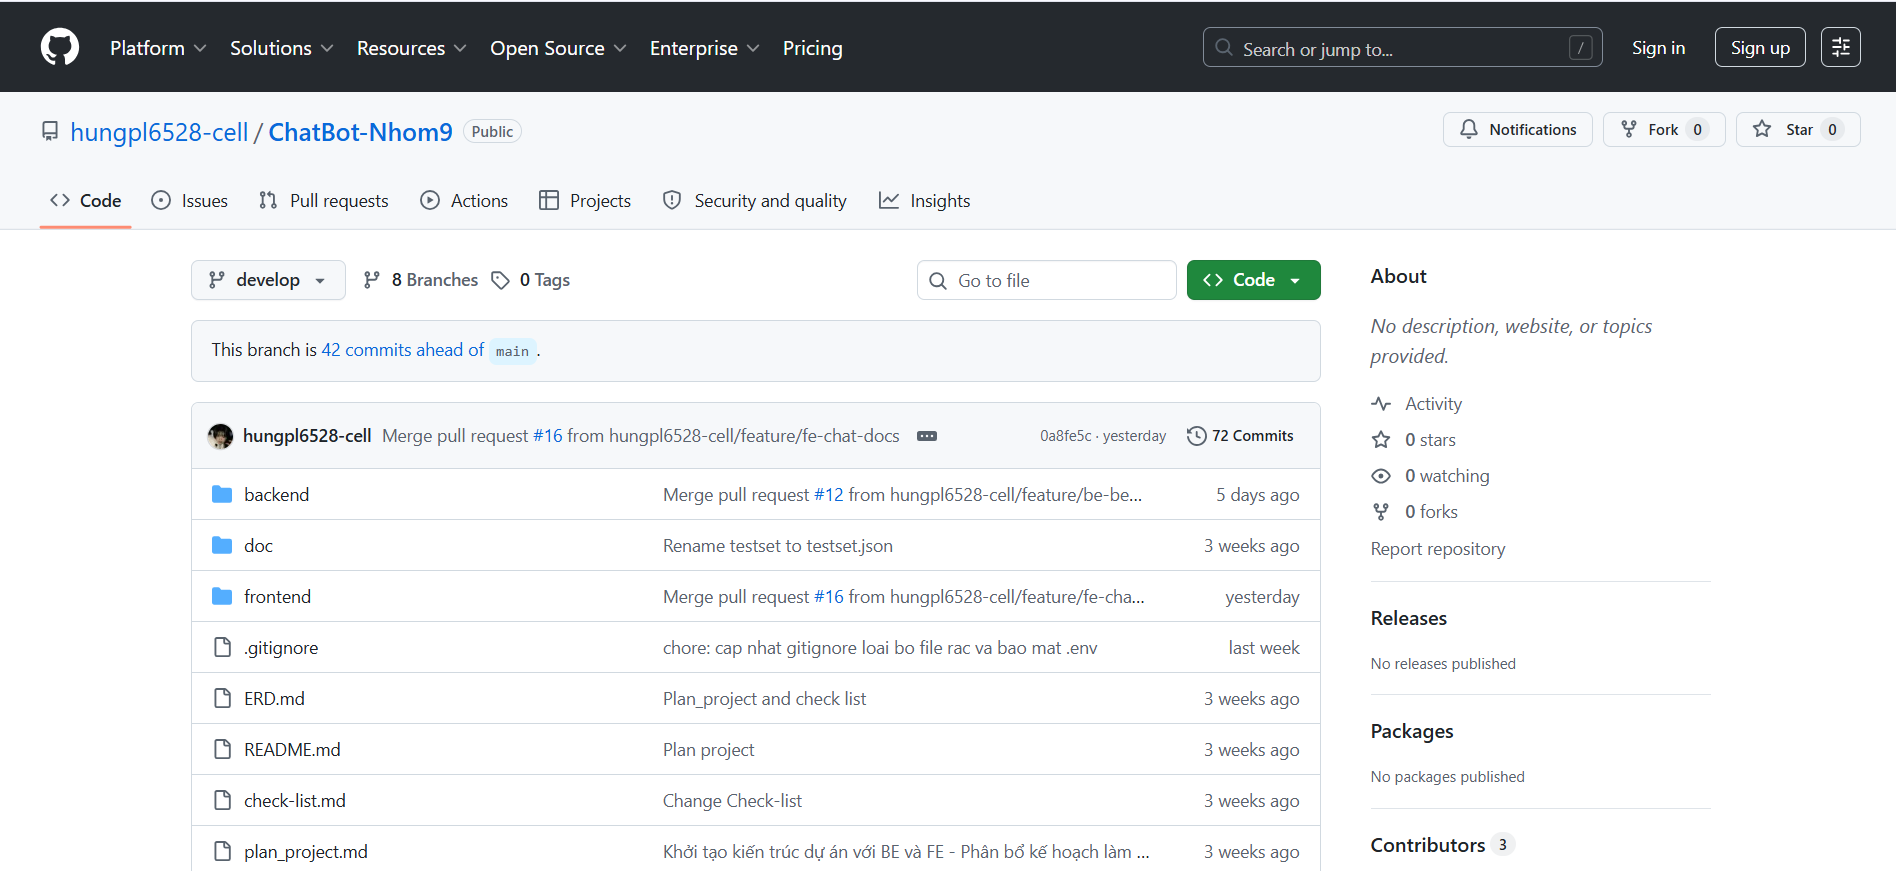
\includegraphics[width=0.95\textwidth]{images/github_repository.png}
  \caption{Repository dự án trên GitHub}
  \label{fig:github-repo}
\end{figure}



Repository được tổ chức thành các thư mục chính:
\begin{itemize}[itemsep=3pt]
  \item \texttt{/backend} -- Mã nguồn FastAPI, các module RAG, Benchmark.
  \item \texttt{/frontend} -- Mã nguồn ReactJS, các component giao diện.
  \item \texttt{/doc} -- Tài liệu dự án (SWP, SWR, SWD, SWT), báo cáo LaTeX.
  \item \texttt{/chromadb\_data} -- Dữ liệu Vector Database.
  \item \texttt{README.md} -- Hướng dẫn cài đặt và chạy dự án.
\end{itemize}

\subsection{Lịch sử Commit}

\begin{figure}[H]
  \centering
  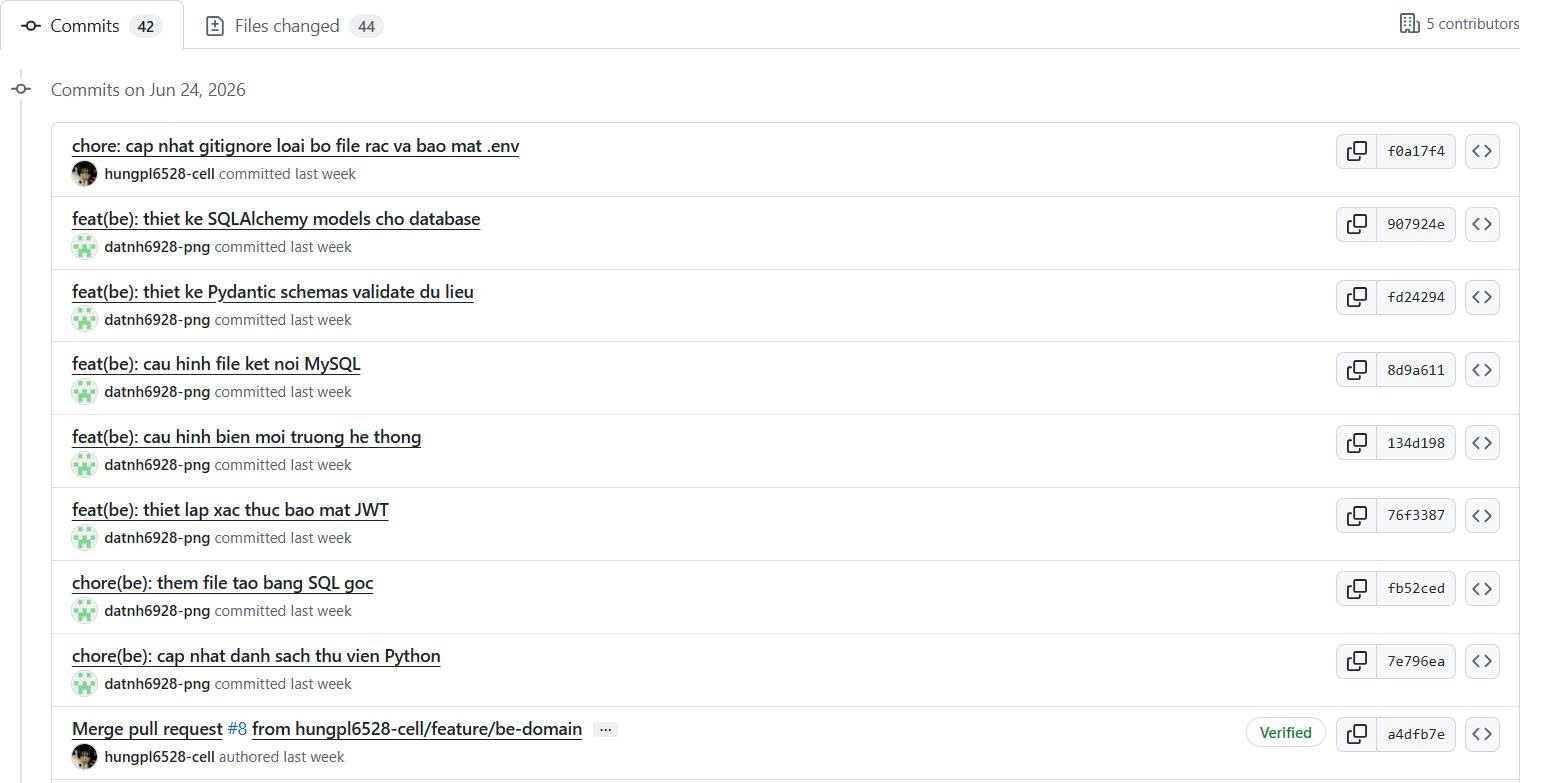
\includegraphics[width=\textwidth]{images/github_commit1.jpg}
  \caption{Lịch sử Commit dự án trên GitHub (Phần 1)}
  \label{fig:commit1}
\end{figure}

\begin{figure}[H]
  \centering
  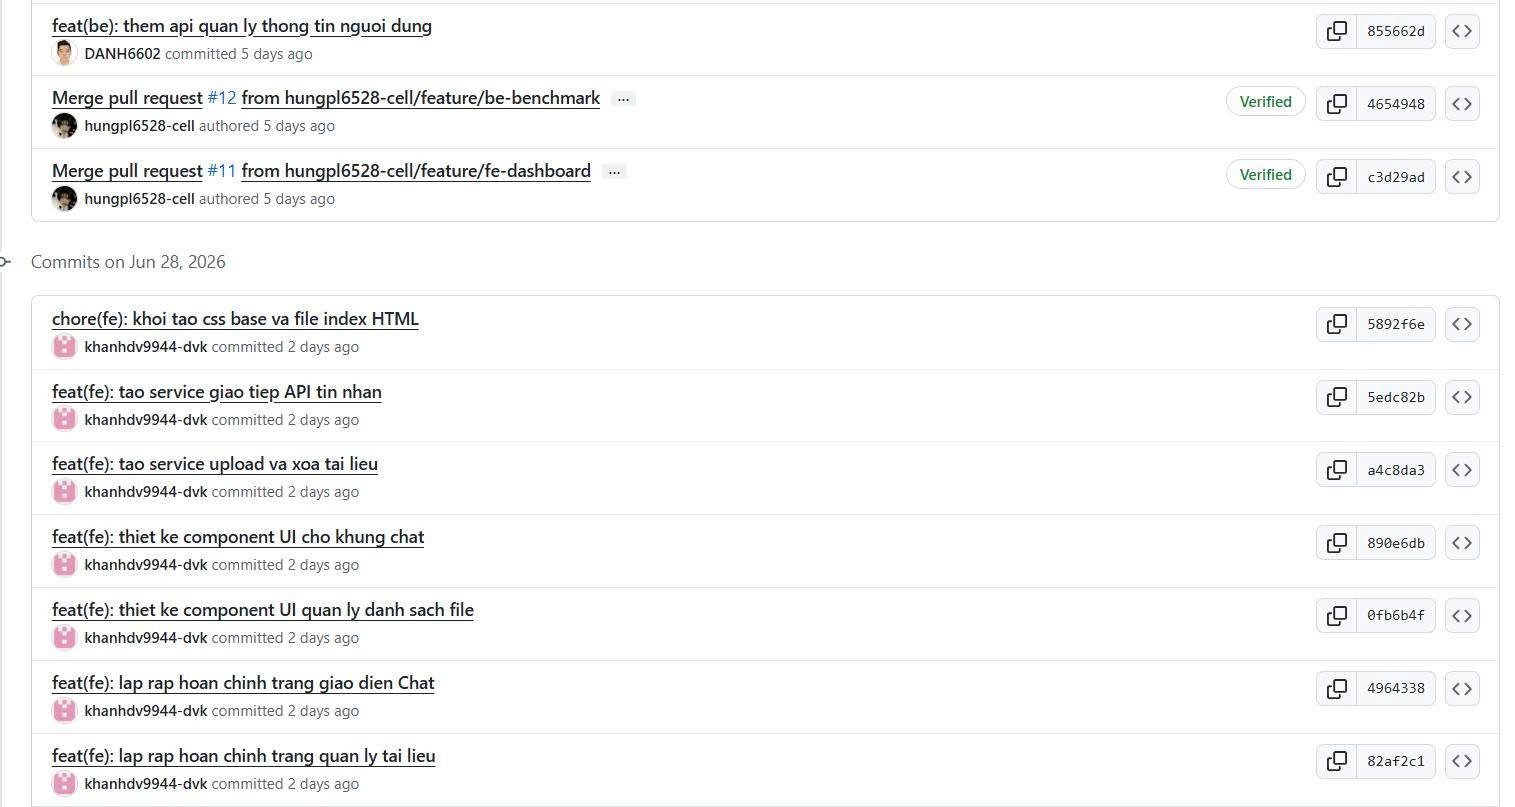
\includegraphics[width=\textwidth]{images/github_commit2.jpg}
  \caption{Lịch sử Commit dự án trên GitHub (Phần 2)}
  \label{fig:commit2}
\end{figure}

\section{Tiêu chuẩn Lập trình}

\begin{table}[H]
  \centering
  \caption{Tiêu chuẩn lập trình áp dụng}
  \label{tab:coding-standards}
  \renewcommand{\arraystretch}{1.4}
  \begin{tabularx}{\textwidth}{|l|l|X|}
    \hline
    \rowcolor{blue!10}
    \textbf{Ngôn ngữ} & \textbf{Tiêu chuẩn} & \textbf{Quy định} \\
    \hline
    Python & PEP 8 & Snake\_case, docstring bắt buộc, max 120 ký tự/dòng. \\
    \hline
    JavaScript & ESLint Airbnb & CamelCase, arrow functions, async/await. \\
    \hline
    SQL & SQL Standard & UPPER CASE cho từ khóa, snake\_case cho tên cột. \\
    \hline
    Git Commit & Conventional Commits & \texttt{feat/fix/docs/test: mô tả ngắn gọn bằng tiếng Anh}. \\
    \hline
  \end{tabularx}
\end{table}

\section{Kết luận Chương}

Chương này đã trình bày đầy đủ kế hoạch quản lý dự án phần mềm (SWP) bao gồm: phạm vi và sản phẩm bàn giao, ước lượng công sức, phân công trách nhiệm (RACI), kế hoạch Sprint theo Agile Scrum, phân tích rủi ro và chiến lược quản lý cấu hình bằng GitHub. Đây là nền tảng để nhóm triển khai dự án một cách có hệ thống, đúng tiến độ và đảm bảo chất lượng.
